% =====================================================================
% Appendix / Backup -- nur bei Fragen in der Diskussion zeigen.
% Seitenzahlen zaehlen nicht zur Gesamtzahl (appendixnumberbeamer).
%
% Neue Backup-Folie anlegen:
%   1. hier: \begin{frame}[label=app-xyz]{Backup: ...} ... \end{frame}
%      mit \buttons{\backto{<label der Hauptfolie>}{Back}}
%   2. auf der Hauptfolie: [label=...] setzen und
%      \buttons{\gotobackup{app-xyz}{Text}}
% =====================================================================

% ---------------------------------------------------------------------
\begin{frame}[allowframebreaks]{References}
  \scriptsize
  \nocite{zschirnt2016,koopmans2019,kline2022,zschirnt2019,adamovic2023}
  \bibliographystyle{apalike}
  \bibliography{\repodir references}
\end{frame}

% ---------------------------------------------------------------------
% A1 <- Folie 7 (Replication)
\begin{frame}[label=app-replication]{Backup: replication with all estimators}
  \slidetable{replication}{0.75\textheight}
  \buttons{\backto{replication}{Back to replication}}
\end{frame}

% ---------------------------------------------------------------------
% A2 <- Folie 10 (Update)
\begin{frame}[label=app-forest]{Backup: forest plot including the new studies}
  \centering
  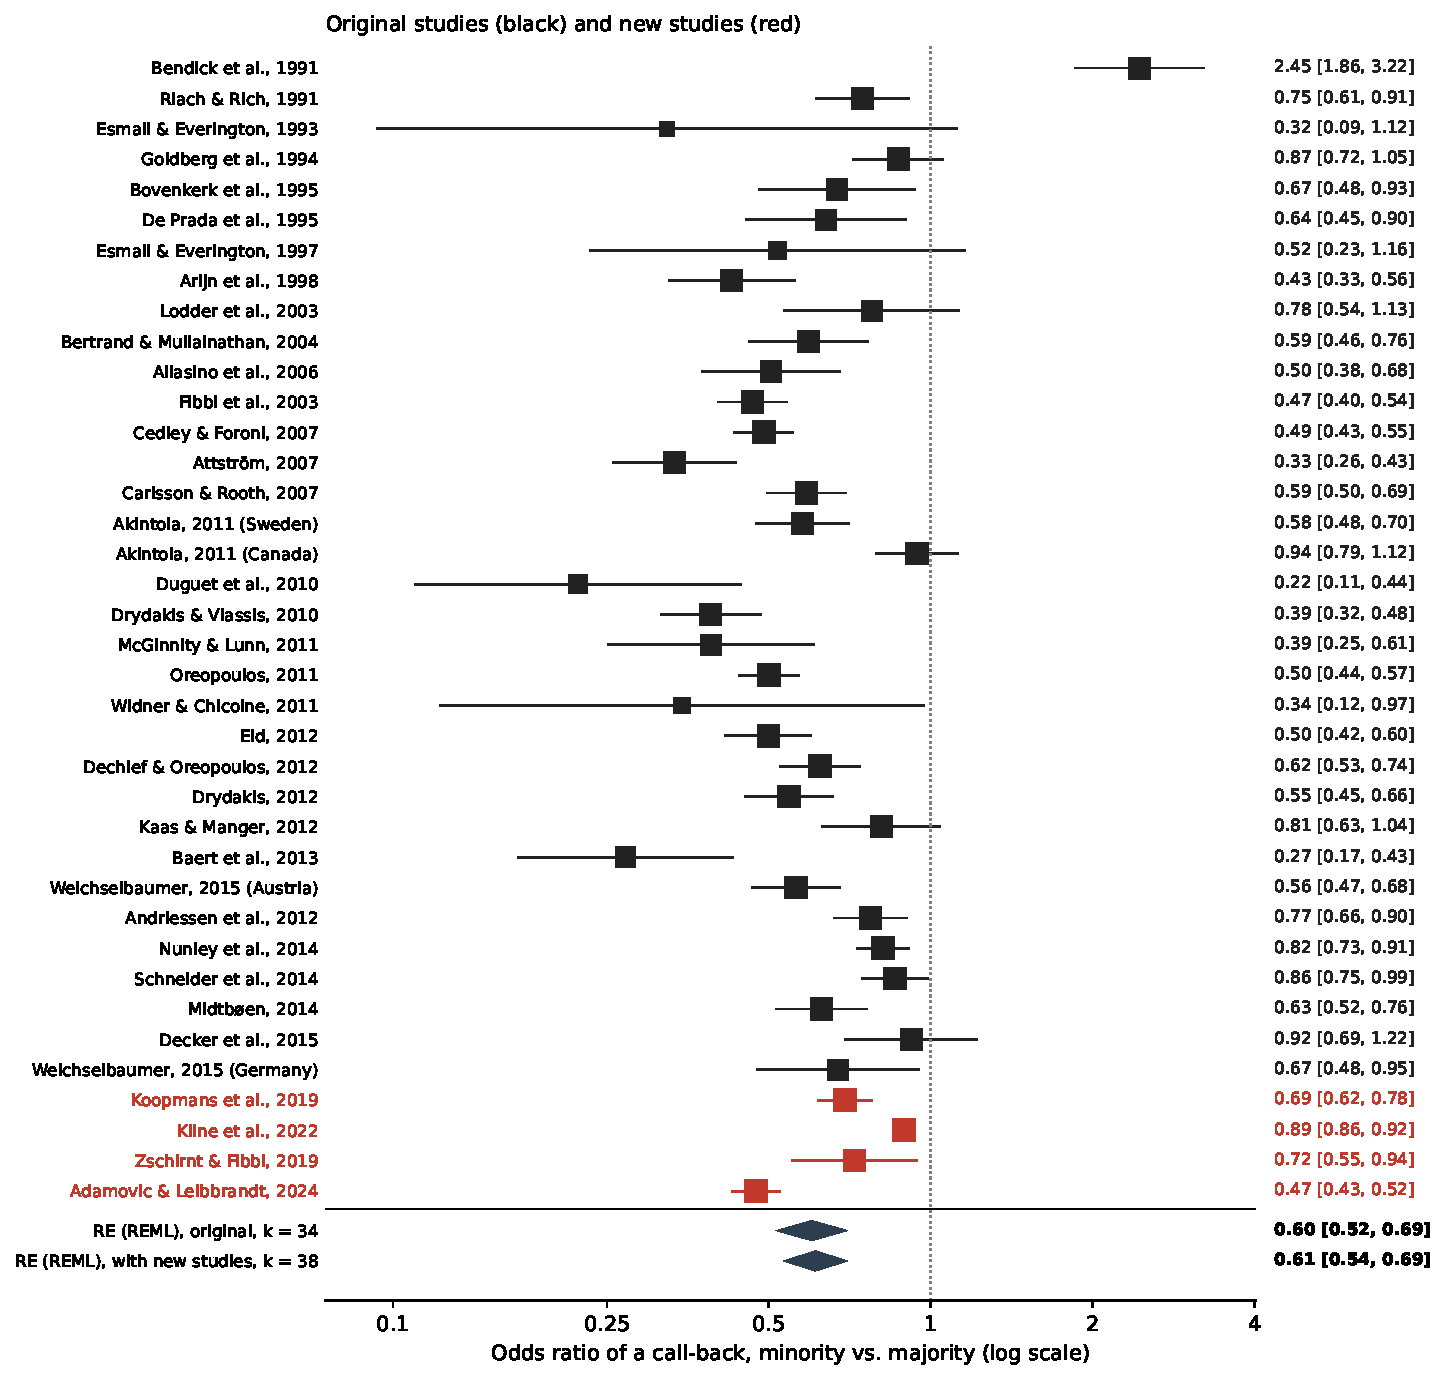
\includegraphics[height=0.8\textheight]{forest_combined}
  \buttons{\backto{update}{Back to update}}
\end{frame}

% ---------------------------------------------------------------------
% A3 <- Folien 10 (Update) und 11 (Power)
\begin{frame}[label=app-power]{Backup: power robustness and the weight of \citet{kline2022}}
  \slidetable{power_robustness}{0.7\textheight}
  \buttons{\backto{update}{Back to update}\quad\backto{power}{Back to power}}
\end{frame}

% ---------------------------------------------------------------------
% A4 <- Folie 13 (Publication bias)
\begin{frame}[label=app-bias]{Backup: pooled and corrected estimates for all samples}
  \slidetable{pubbias_estimates}{0.72\textheight}
  \buttons{\backto{bias}{Back to publication bias}}
\end{frame}
